%
%% Kapitel: Kapitel 4
%%======================================================================

\chapter{Klassifikation von Geschwindigkeitsbodenmarkierungen}
\label{cha:Klassifikation von Geschwindigkeitsbodenmarkierungen} \index{Klassifikation von Geschwindigkeitsbodenmarkierungen}
%
%


\section{Aufbau des Machine-Learning Frameworks}
\label{sec:Aufbau des Machine-Learning Frameworks}

Bei der Wahl der Programmiersprache fiel die Wahl auf Python. Es ist eine Objektorientierte Programmiersprache die sich vorallem im Wissenschaftlichen Bereich immer mehr beliebtheit erfeut. Vorallem im Datascience und Machine Learning Umfeld findet Python h{\"a}ufig seine Anwendung. Durch seine dynamische Datentypverwaltung und der Strukturierung durch Einr{\"u}cken des Codes ist er sehr {\"u}bersichtlich. Zudem stehen viele Software-Module durch die gro{\ss}e Python-Community zur Verf{\"u}gung was Python zu einem sehr m{\"a}chtigen Werzeug macht.
F{\"u}r das integrieren der Module zu einem gesamtsystem wurde die Anaconda Python/R Data Science Platform genutzt. Sie beihnalten den Conda Paketmanager welcher eine gro{\ss}e Unterst{\"u}tzung beim finden und installieren von Softwarepaketen ist. Auch werden abh{\"a}ngigkeiten von verschiedenen Softwareversion der Module automatisch durch Conda gel{\"o}st was sonst oft zu Problemen gef{\"u}hrt hat. Conda ist auch ein Umgebungsmanager mit dem Software lokal abgetrennt in einer eigenen Umgebung programmiert werden kann. Dies ist n{\"u}tzlich wenn etwa Verschiedene Python Versionen auf dem selben System genutzt werden m{\"u}ssen.
Im Folgenden sind die Python-Module aufgelistet die in der Arbeit ihre Verwendung fanden.

\begin{enumerate}

\item[] \textbf{Pycharm}\hfill \\
Pycharm ist eine integrierte Entwicklungsumgebung f{\"u}r Python. 
Sie assisitiert beim Programmieren durch, Codevervollst{\"a}ndigung sowie syntax und Fehler Hervorhebung. Der Hauptgrund f{\"u}r die Wahl dieser IDE war der effizeinte Python-Debugger durch den man auch beim Arbeiten auf gro{\ss}en Datenstrukturen einen leichten {\"U}berblick {\"u}ber das Verhalten des Codes bekommt.


\item[] \textbf{Numpy}\hfill \\
Die Programmbibliothek Numpy steht f{\"u}r Numeric Python. Sie bietet funktionen zum arbeiten mit gro{\ss}en Arrays und Matrizen. Auch numerische Berechnungen und mathematische Routinen sind implementiert. Da viele Numpy-Operationen in C implementiert sind hat die Bibliothek auch eine gute Performance.


\item[] \textbf{Matplotlib}\hfill \\
Durch Matplotlib lassen sich Mathematische zusammenh{\"a}nge oder Daten visualisieren. 
Mit nur wenigen Codezeilen lassen sich zum Beispiel Histogramme, Balkendiagramme, Korrelationsdiagramme oder Punktwolken visualisieren. Die Bibliothek ist eine kostenfreie alternative zur visualisierung mit Matlab.


\item[] \textbf{Pandas}\hfill \\
Pandas ist eine Python-Paket welches zur Datenanalyse und verarbeitung von Daten genutzt wird.
Vorallem die DataFrames eine zweidimensionale Datenstruktur welche Spalten mit verschiedenen Datentypen beinhalten kann sind sehr n{\"u}tzlich zur vorverarbeitung von Datens{\"a}tzen f{\"u}r das maschinelle lernen. Eine Speicherstelle kann einfach {\"u}ber ihren Spaltenname und den Zeilenindex angepsrochen werden. Es lassen sich schnell Statistiken {\"u}ber einzelne oder mehrer Spalten berechnen oder einzelne Ausrei{\ss}er lokalisieren. Auch das lesen und speichern von zum Beispiel CSV, Text-Dateien oder SQL-Datenbanken ist gegeben.

\item[] \textbf{Scikit-learn}\hfill \\
Scikit-Learn ist eine Software-Bibliothek zum maschinellen Lernen f{\"u}r Python.
Sie bietet verschiedene Klassen von Algorithmen an. Diese sind Regressions-, Klassifikations sowie Clusteralgorithmen. Es werden auch Funktionen zur Aufbereitung von 
Datens{\"a}tzen angeboten da manche Verfahren andere Representationen von Trainingsdaten ben{\"o}tigen um effizient lernen zu k{\"o}nnen. Weiter bieten Scikit-Learn Metriken zur Bewertung von trainierten Modellen. Viele Kernfunktionen sind in Cython geschrieben um die Dauer des Trainings zu beschleunigen. Eine beschleunigung durch GPUs ist nicht implementiert. Alle Berechnungen finden auf dem Hauptprozessor statt.

\item[] \textbf{Tensorflow}\hfill \\
Tensorflow ist ein Framework f{\"u}r das maschinelle Lernen entwickelt von Google.
Es wird vorallem zum Training von Deep-Learning Architekuren verwendet.
Rechenschritte werden als Datenflussgraphen dargestellt um Abh{\"a}ngigkeiten zwischen einzelnen Operationen zu representieren.
Durch die NVIDIA-CUDA Erweiterung von Tensorflow k{\"o}nnen Berechnungen durch GPUs hoch parallelisiert werden und mit der zus{\"a}tzlichen Programmierbibliothek NVIDIA-cuDNN wird es
erm{\"o}glicht auch K{\"u}nstliche Neuronale Netze GPU-beschleunigt zu optimieren.
\item[] \textbf{Keras}\hfill \\
Keras ist eine Deep-Learning Bibliothek und High-Level API. Es ist die Schnittstelle f{\"u}r verschiedene Backends wie Tensorflow oder Theano. Die API hat eine hohe Bedienerfreundlichkeit nd erm{\"o}glicht ein schnelles und einfaches Prototyping von neuronalen Netzen.
\item[] \textbf{Jupyter-Notebook}\hfill \\
Jupyter-Notebook ist eine Webapplikation die es erlaubt den Code und dessen Dokumentation in einer geteilten Umgebung zu verwenden. Es wird gerne in Datascience Projekten genutzt. Sehr n{\"u}tzlich sind sie falls man sich noch in der Protoypenphase befindet. Code wird in verschiedenen Zellen aufgef{\"u}hrt dies erlaubt es einen bestimmten Code-Block auszuf{\"u}hren ohne das Gesamte Programm neuzustarten.  Dadurch m{\"u}ssen Daten nicht immer wieder erneut in den RAM geladen werden oder es k{\"o}nnen Parameter beim Training von ML-Modellen flexibel angepasst werden. Auch bei der Visualisierung von Daten ist es hilfreich.



\end{enumerate}


\section{Klassifikation durch Template Matching}
\label{sec:Klassifikation durch Template Matching}

Da die Geschwindigkeitsmarkierungen auf der Fahrbahn immer gleich aussehen wurde sich dazu entschieden, die Markierungen {\"u}ber ein Template-Matching zu klassifizieren.
Daf{\"u}r wird die OpenCV-Funktion MatchTemplate verwendet.
Die Bilder f{\"u}r das Template-Matching wurden aus der Simulation heraus extrahiert und extern abgespeichert. Zur Laufzeit des Programms werden die Templates in das Programm eingeladen.

\begin{figure}[H]
\begin{center}
  
\includegraphics[width=0.8\textwidth]{/home/tb/gazebo_road_generation/02_Arbeit_Latex/009_Kapitel8/Bilder/roadspeedsigngs}% keine extention: wählt jpg für DVI
  \caption[Geschwindigkeitsmarkierungstemplates]%
           {\label{fig:Geschwindigkeitsmarkierungstemplates}%
           Geschwindigkeitsmarkierungstemplates.
           }
\end{center}
\end{figure}

Die Templates haben eine Dimension von XXX welche genau derselben Gr{\"o}{\ss}e der Geschwindigkeitsmarkierungen in der Simulation in Birdseye-Perspektive entsprechen. Das Bild auf dem TemplateMatch angewandt wird, wird aus der Topic /road\_sign ausgelesen.
Die Funktion MatchTemplate faltet das Template {\"u}ber den Bildbereich und berechnet einen Score abh{\"a}ngig von der ausgew{\"a}hlten Methode. Folgende Methoden wurden getestet.

\begin{enumerate}

\item[] \textbf{CV\_TM\_SQDIFF}\hfill \\
Berechnet die euklidische Distanz nach folgender Formel:

\begin{figure}[H]
\begin{center}
  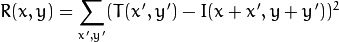
\includegraphics[width=0.8\textwidth]{/home/tb/gazebo_road_generation/02_Arbeit_Latex/009_Kapitel8/Bilder/sqdiff}% keine extention: wählt jpg für DVI
  \caption[SQDIFF]%
           {\label{fig:SQDIFF}%
           Berechnung der euklidischen Distanz zwischen Pixel und Template.
           }
\end{center}
\end{figure}


\item[] \textbf{CV\_TM\_CCORR}\hfill \\
Berechnet die Korrelation nach folgender Formel:

\begin{figure}[H]
\begin{center}
  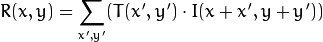
\includegraphics[width=0.8\textwidth]{/home/tb/gazebo_road_generation/02_Arbeit_Latex/009_Kapitel8/Bilder/ccorr}% keine extention: wählt jpg für DVI
  \caption[CCORR]%
           {\label{fig:CCORR}%
           Berechnung der korrelation zwischen Pixel und Template.
           }
\end{center}
\end{figure}

\end{enumerate}

Die Ausgabe von MatchTemplate ist eine OpenCV-Matrix mit den Werten der Aktivierungen durch das Falten mit dem entsprechenden Template.
Bei der Methode CV\_TM\_SQDIFF gibt der minimale Wert in der Matrix den besten Score an. Bei der Methode CV\_TM\_CORR gibt der maximale Wert den besten Score an. Diese werden mit der OpenCV-Funktion minMaxLoc ermittelt.
Alle neun Scores der Templates werden mit dem Bild aus /road\_sign berechnet.
Das Template mit dem besten Score steht f{\"u}r die klassifizierte Geschwindigkeitsmarkierung. 



\section{Aufbereitung des MNIST-Trainingsdatensatzes}
\label{sec:Aufbereitung des MNIST-Trainingsdatensatzes}

F{\"u}r das training der Machine-Learning Modelle zur Klassfikation der Geschwindigkeitsbodenmarkierungen wurde der MNIST-Datensatz verwendet.
Dieser Besteht aus einem Trainingsdatensatz mit 60000 Handgeschriebenen einstelligen Ziffern von null bis neun mit einer Dimension von 28x28. Und einem zugeh{\"o}rigen Testdatensatz mit 10000 Ziffern.
Da die Geschwindigkeitsmarkierungen beim Carolo-Cup nur zweistellige Zahlen beeinhalten wurden die nullen aus dem Datensatz zuf{\"a}llig an die Zahlen eins bis neun angeh{\"a}ngt. Dadurch ergibt sich eine Bilddimension von 28x56 mit dem die verschiedenen Machine-Learning Modelle trainiert wurden.

\begin{figure}[H]
\begin{center}
  
\includegraphics[width=1.0\textwidth]{/home/tb/gazebo_road_generation/02_Arbeit_Latex/009_Kapitel8/Bilder/mnist}% keine extention: wählt jpg für DVI
  \caption[Aufbereitete Features des MNIST-Datensatzes]%
           {\label{fig:Aufbereitete Features des MNIST-Datensatzes}%
           Aufbereitete Features des MNIST-Datensatzes.
           }
\end{center}
\end{figure}

\section{Klassifikation durch Random Forest}
\label{sec:Klassifikation durch Random Forest}

Random Forest ist ein {\"u}berwacht trainiertes maschinelles Lernverfahren welches aus einem Ensemble von randomisiert trainierten Entscheidungsb{\"a}umen besteht. Entwickelt wurde das Verfahren 2001 durch Leo Breiman. Es ist m{\"o}glich den Algorithmus als Klassifikiationsansatz oder als Regressionsansatz zu implementieren. Bei der Auswertung von Random Forest wird die Entscheidung nach einem Mehrheitsvotum durch die einzelnen Entscheidungsb{\"a}ume getroffen.
Random Forest ist eines der am h{\"a}ufigsten genutzten Algorithmen zur Auswertung von Daten. Es liefert sehr gute Ergebninsse auf verschiedenste Datens{\"a}tze und hat eine geringe Trainingszeit im vergleich zu neuronalen Netzen. Das Verfahren kann mit tausenden von Eingangsvariablen umgehen und es sind bin{\"a}re kategoriale als auch numerische Merkmals-Typen lernbar.
Zudem ist das Verfahren robust gegen {\"U}beranpassung durch das training der einzelnen B{\"a}ume mit Boostrap-Stichprobieren und des Mehrheitsvotums bei der Entscheidungsf{\"a}llung. 
Random Forest kommt auch mit outliern und unstandardisierten Daten zurrecht.
Auch ist es m{\"o}gliche ein Einsehen in das trainierte Modell zu bekommen. Dadurch kann die prozentuale wichtigkeit einzelner Trainingsmerkmale bei der Entscheidungsfinding erhalten werden.

\subsection{Aufbau eines Entscheidungsbaums}
\label{subsec:Aufbau eines Entscheidungsbaums}

Ein Entscheidungsbaum wird umgekehrt mit seiner Wurzel an der Spitze dargestellt.
Sie sind aus einer Kombinaition von vier Komponenten aufgebaut.


\begin{enumerate}

\item[] \textbf{Wurzelknoten}\hfill \\
Stellt den Input des Baumes dar und f{\"a}llt die erste Entscheidung zur Separation der Eingangsdaten.

\item[] \textbf{Innere Knoten}\hfill \\
Beeinhalten logische Tests welche durch ein {\"u}berwachtes Training spezifiziert wurden


\item[] \textbf{Bl{\"a}tter}\hfill \\
Sie sind das Ende des Baumes und stehen f{\"u}r das Ergebnis der Klassifikation.

\item[] \textbf{Kanten}\hfill \\
Verbindung zwischen Wurzelknoten, Innerer Knoten und Bl{\"a}ttern
\end{enumerate}


Vom Wurzelknoten aus wird der Merkmalsvektor einer Oberservation durch den Baum gef{\"u}hrt bis er an einem Blatt angelangt ist. Dadurch wird die Oberservation klassifiziert.
Der Weg der {\"u}er die Kanten und inneren Knoten durchlaufen wird ist abh{\"a}ngig von den logischen Tests.



\begin{figure}[H]
\begin{center}
  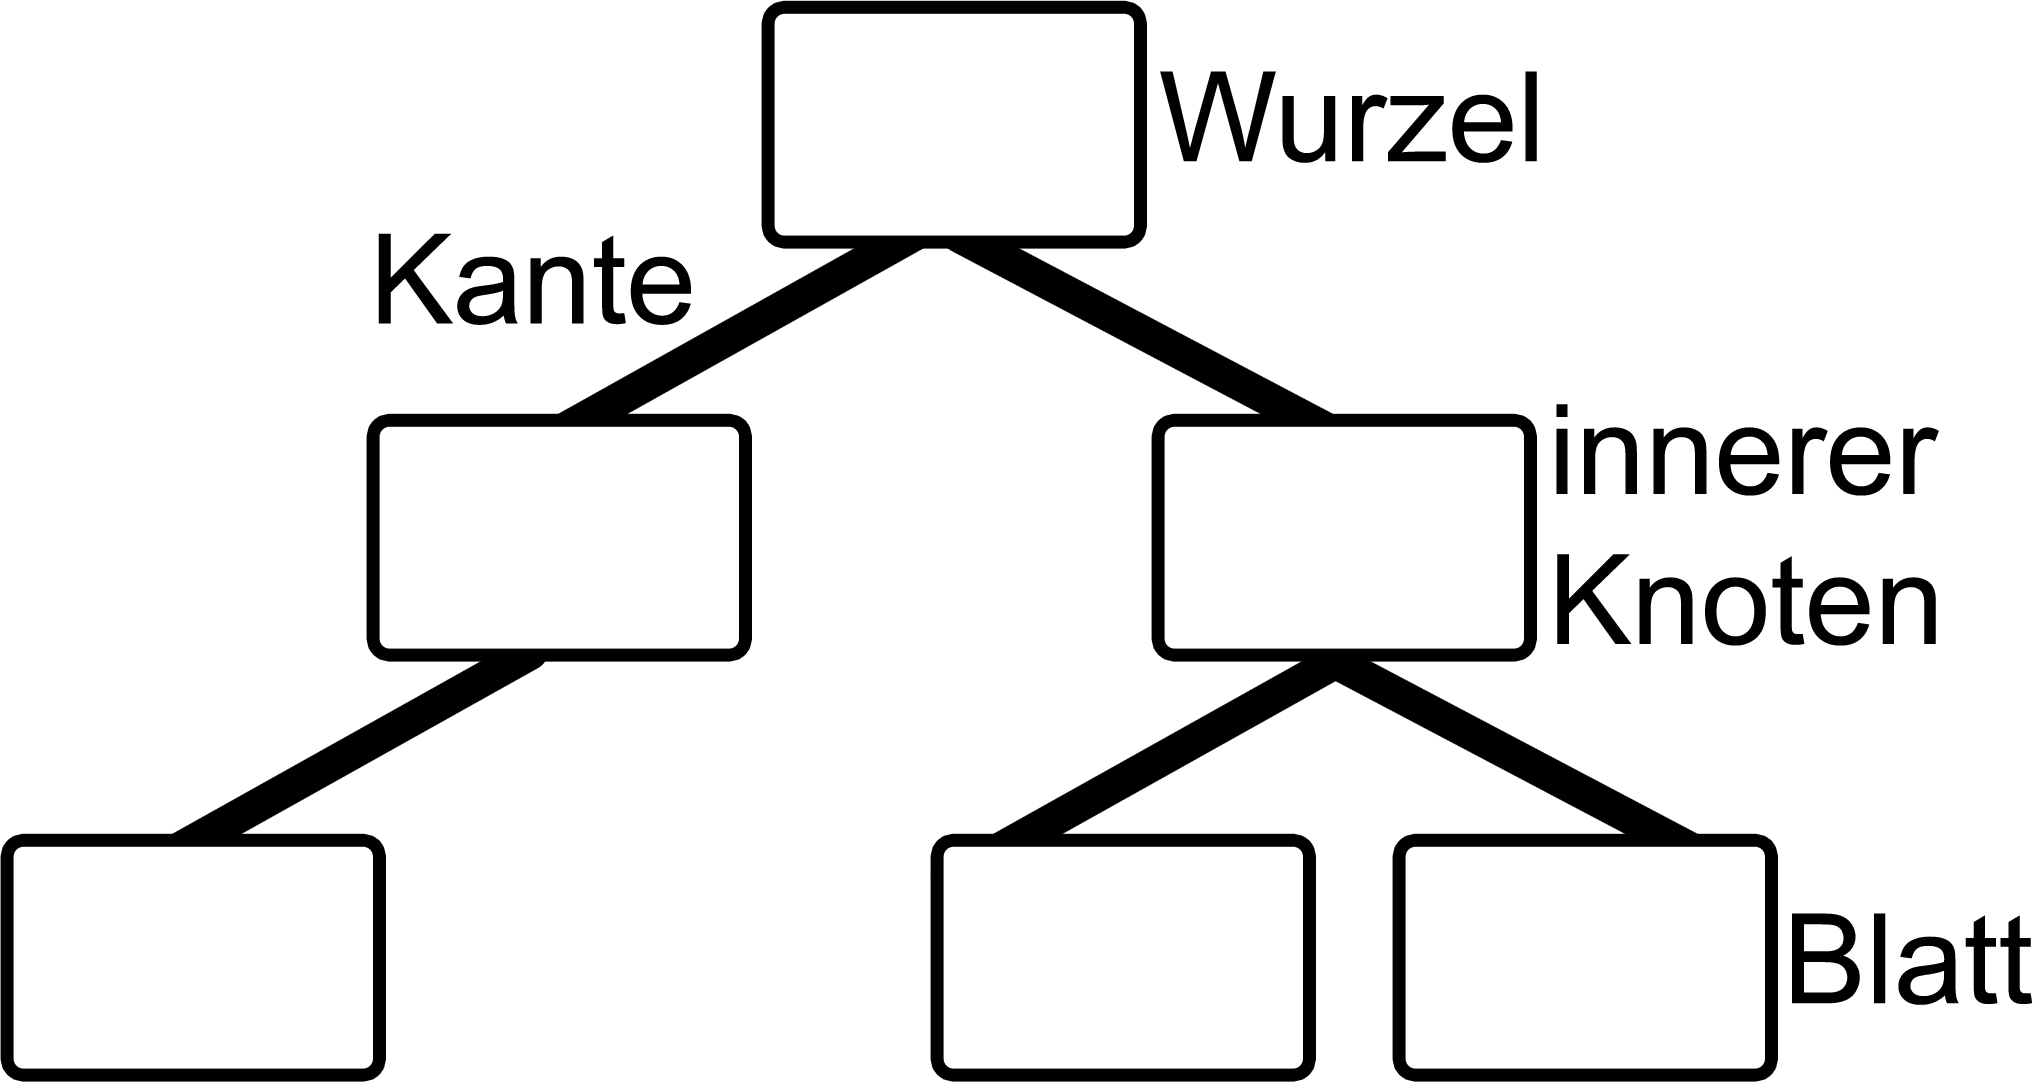
\includegraphics[width=0.5\textwidth]{/home/tb/gazebo_road_generation/02_Arbeit_Latex/009_Kapitel8/Bilder/tree}% keine extention: wählt jpg für DVI
  \caption[Aufbau eines Entscheidungsbaums]%
           {\label{fig:Aufbau eines Entscheidungsbaums}%
           Aufbau eines Entscheidungsbaums.
           }
\end{center}
\end{figure}

Der CART-Algorithmus (Classification and Regression Tree) ist ein Verfahren um die logischen Tests der Knoten zur korrekten Klassifikation zu lernen. Die Modellstruktor des Entscheidungsbaumes ist dabei nicht von vorneherin festgelegt sondern wird durch die Daten bestimmt. 
Beim training des Algorithmus werden N Samples von Observationen mit Merkmals-Vektoren und bekannten Labeln zuf{\"a}llig aus dem gesamten Datensatz mit der selben gr{\"o}{\ss}e N  ausgew{\"a}hlt. Bei der Auswahl kann auch die selbe Observation mehrmals gezogen werden. Dies Wird  Bootstrapping genannt. 
F{\"u}r jeden Entscheidungsbaum des Random Forest Algorithmus wird ein zuf{\"a}lliges Subset von Merkmalen ausgew{\"a}hlt. Bei M Input-Merkmalen also m<M Merkmale die f{\"u}r jeden einzelnen Entscheidungsbaum konstant gehalten werden. Bei der Klassifikation wird meist die Wurzel aus der Anzahl der gesamten Merkmale genommen m = sqrt(M) [vgl. Hastie et al., S. 592 [16]]. Dies ist ein weiterer Trick um dem Algorithmus eine bessere Generalisierung zu verschaffen da dadurch die Entscheidungsb{\"a}ume weniger miteinander korrelieren.
Der CART-Algorithmus in jedem Schritt anhand eines der zuf{\"a}llig ausgew{\"a}hlten Merkmale durch einen logischen Test das Set in zwei getrennte Gruppen aufzuteilen (bin{\"a}rer Split).

Um das Merkmal zu finden welches die Daten am besten teilt wird das Gini-Unreinheitsma{\ss} verwendet. Es gibt an wie Wahrscheinlich es ist einen Datenpunkt falsch zu klassifizieren.
Hat man J verschiedene Klassen ist  p(i) die Wahrscheinlichkeit einen Datenpunkt der Klasse i zu w{\"a}hlen. Somit Berechnet sich das Gini-Unreinheitsma{\ss} nach folgender Formel:

\begin{figure}[H]
\begin{center}
  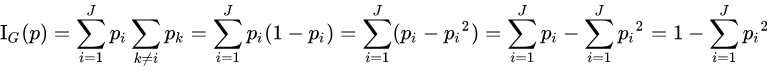
\includegraphics[width=1.0\textwidth]{/home/tb/gazebo_road_generation/02_Arbeit_Latex/009_Kapitel8/Bilder/gini}% keine extention: wählt jpg für DVI
  \caption[Formel zur Berechnung des Gini-Unreinheitsmass]%
           {\label{fig:Formel zur Berechnung des Gini-Unreinheitsmass}%
           Formel zur Berechnung des Gini-Unreinheitsmass.
           }
\end{center}
\end{figure}

Die Berechnung eines Splits wird folgend an einem Beispiel veranschaulicht.
Angenommen man habe drei verschiedene Klassen mit insgesamt 80 Observationen welche Merkmale und zugeh{\"o}rige Klassen in sich vereinen.
Davon befinden sich 19 Observationen in der Klasse eins, 21 Observationen in der Klasse zwei und 40 Observationen in der Klasse drei. Das Gini-Unreinheitsma{\ss) berechnet sich nun zu:


$1- [ (\frac{19}{80})^2 + (\frac{21}{80})^2 + (\frac{40}{80})^2] = 0,6247$


Um den logischen Test f{\"u}r den besten bin{\"a}ren Split {\"u}ber ein Merkmal der Observationen zu finden werden die Gini-Unreinheitsma{\ss)e f{\"u}r alle m{\"o}glichen Werte durchgetestet.
Angenommen man w{\"u}rde das Merkmal X1 bei X1 > 2 aufteilen und die Observationen w{\"u}rden sich nach Klassen folgederma{\ss)en aufteilen:

Linke Kante: 16, 9, 0\\
Rechte Kante : 3, 12, 40

Dann errechnet sich das Gini-Unreinheitsma{\ss} zu:

Linke Kante:   $1 - [ (\frac{16}{25})^2 + (\frac{9}{25})^2] = 0,4608$\\
Rechte Kante: $1 - [ (\frac{3}{55})^2 + (\frac{12}{55})^2+ (\frac{40}{55})^2] = 0,4205$

Um die Qualit{\"a}t des Splits zu beurteilen werden die Unreinheitsma{\ss)e je Kante mit der Anzahl in Sie hinfeinfallender Observationen Gewichtet und die Werte gemittelt. 
Dies ergibt das mittlere Gewichtete Unreinheitsma{\ss) f{\"u}r den Split X1 > 2.

$\frac{25}{80} * Gini Linke Kante + \frac{55}{80} * Gini Rechte Kante = 0,4331$

Der Gewinn des Splits kann nun berechnet werden indem das Gini-Unreinheitsma{\ss) nach dem Split von dem Gini-Unreinheitsma{\ss) vor dem Split subtrahiert wird. Dieser Wert wird auch Gini-Gain genannt. 

$0,6247 - 0,4331 = 0,1916$

Der Split der die Observationen mit dem gr{\"o}{\ss)ten Gewinn aufteilt wird anschlie{\ss)end im Entscheidungsbaum verwendet und es findet ein neuer Split f{\"u}r jede Kante statt.
Dies wird wiederholt bis ein festgelegtes Stoppkriterium erreicht ist oder in eine Kante nurnoch eine Observation f{\"a}llt. Alle Knoten die nichtmehr gesplittet werden, werden zu Bl{\"a}ttern.
Ein Blatt steht am Ende des durch Trainings gewachsenen Baumes f{\"u}r jene Klasse welche am h{\"a}ufigsten in sie hineinf{\"a}llt.

\begin{figure}[H]
\begin{center}
  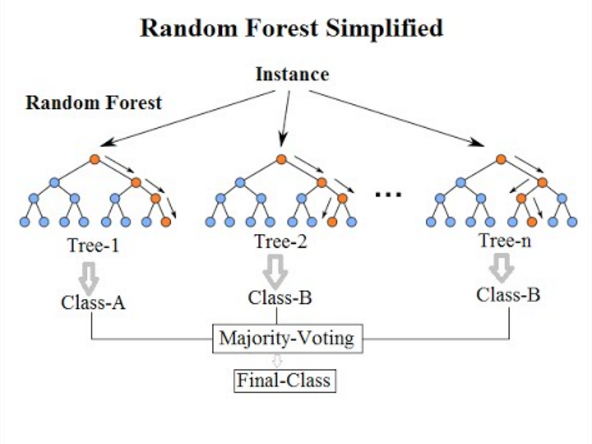
\includegraphics[width=1.0\textwidth]{/home/tb/gazebo_road_generation/02_Arbeit_Latex/009_Kapitel8/Bilder/rfm}% keine extention: wählt jpg für DVI
  \caption[Ein Random Forest Modell]%
           {\label{fig:Ein Random Forest Modell}%
           Ein Random Forest Modell.
           }
\end{center}
\end{figure}
